\section{Адаптация тензорного алгоритма для Points-to анализа, учитывающего поля}

% Расписать, почему матричный алгоритм плохо подходит
%Алгоритм, основанный на умножении матриц, требует создания булевой матрицы смежности для каждого нетерминала грамматики, поэтому для его практического применения необходимо, чтобы число нетерминалов грамматики в ослабленной нормальной форме Хомского было не очень велико.
Для практического применения алгоритма, основанного на умножении матриц, желательно, чтобы число нетерминалов грамматики в ослабленной нормальной форме Хомского было не очень велико, поскольку для каждого из них требуется создать булеву матрицу смежности. %енто перефразированное предложение
Например, в грамматике для анализа псевдонимов, переведённой в ослабленную нормальную форму Хомского, 12 нетерминалов. Однако число продукций в грамматике для Points-to анализа, учитывающего поля, зависит от числа полей анализируемой программы и может достигать нескольких тысяч. Это делает матричный алгоритм плохо применимым.

% Расписать, почему тензорный алгоритм алгоритм плохо подходит
В алгоритме, основанном на произведении Кронекера, для пересечения рекурсивного автомата и ориентированного графа они представляются как композиция булевых матриц смежности для всех различных меток на рёбрах. На рис.~\ref{fig:java_rsm} представлен рекурсивный автомат для Points-to анализа, учитывающего поля. Можно заметить, что все метки на рёбрах, кроме Alias, встречаются по одному разу.
%Поэтому для всех этих меток будет создана булева матрица смежности, содержащая единственный элемент, для всех этих матриц необходимо считать произведение Кронекера с соответствующей матрицей смежности графа, а затем складывать полученный результат.
Поэтому для всех этих меток будет создана булева матрица смежности, содержащая единственный элемент, и для каждой из них необходимо считать произведение Кронекера с соответствующей матрицей смежности графа, а затем складывать полученный результат.%хз, насколько удачно убран повтор "матриц"

\begin{figure}[h]
  \begin{tabular}{|c|c|c|}
    \hline
    PointsTo & FlowsTo & Alias \\
      % Программа & Граф выражений \\
      
      \begin{minipage}{.37\textwidth}
      \scalebox{0.6}{
      \begin{tikzpicture}[node distance=1.9cm, auto] 
          \node (q0) [state, initial, initial text = {}] {$q_0$};
          \node (q1) [state, accepting, below = of q0] {$q_1$};
          
          \node (q4) [right = of q0] {$...$};
          
          \node (q2) [state, above = of q4] {};
          \node (q3) [state, right = of q2] {};
          
          \node (q5) [state, below = of q4] {};
          \node (q6) [state, right = of q5] {};
          
          \path [-stealth, thick]
              (q0) edge [loop above]  node[above left] {$assign$}()
              (q0) edge node[left] {$alloc$} (q1)
              
              (q0) edge[bend left] node[below right] {$load_{f_1}$} (q2)
              (q2) edge node[above] {$Alias$} (q3)
              (q3) edge node[below right] {$store_{f_1}$} (q0)
              
              (q0) edge[bend right] node[above right] {$load_{f_n}$} (q5)
              (q5) edge node[above] {$Alias$} (q6)
              (q6) edge node[above right] {$store_{f_n}$} (q0)
              ;
      \end{tikzpicture}
      }
      \end{minipage}
  
      &
  \begin{minipage}{.38\textwidth}
  \scalebox{0.6}{
      \begin{tikzpicture}[node distance=1.9cm] 
          \node (q0) [state, initial, initial text = {}] {$q_2$};
          \node (q1) [state, accepting, below = of q0] {$q_3$};
          
          \node (q4) [right = of q1] {$...$};
          
          \node (q2) [state, above = of q4] {};
          \node (q3) [state, right = of q2] {};
          
          \node (q5) [state, below = of q4] {};
          \node (q6) [state, right = of q5] {};
          
          \path [-stealth, thick]
              (q0) edge node[left] {$\overline{alloc}$} (q1)
              (q1) edge [loop below] node[below left] {$\overline{assign}$}()
              
              (q1) edge[bend left] node[below right] {$\overline{store_{f_1}}$} (q2)
              (q2) edge node[above] {$Alias$} (q3)
              (q3) edge node[below right] {$\overline{load_{f_1}}$} (q1)
              
              (q1) edge[bend right] node[above right] {$\overline{store_{f_n}}$} (q5)
              (q5) edge node[above] {$Alias$} (q6)
              (q6) edge node[above right] {$\overline{load_{f_n}}$} (q1);
      \end{tikzpicture} 
      }
      \end{minipage}
      &
  \begin{minipage}{.17\textwidth}
  \scalebox{0.7}{
      \begin{tikzpicture}[node distance=1.0cm] 
          \node (q0) [state, initial, initial text = {}] {$q_4$};
          \node (q1) [state, below = of q0] {$q_5$};
          \node (q2) [state, accepting, below = of q1] {$q_6$};
          \path [-stealth, thick]
              (q0) edge node[right] {$PointsTo$} (q1)
              (q1) edge node[right] {$FlowsTo$} (q2)
              ;
      \end{tikzpicture} 
      }
      \end{minipage}
      \\
      & & \\
      \hline
  
  \end{tabular}
  \caption{Рекурсивный автомат для Points-to анализа, учитывающего поля}
  \label{fig:java_rsm}
\end{figure}

% Расписать, как улучшили тензорный алгоритм
С целью уменьшения числа операций был рассмотрен другой способ представления графа и рекурсивного автомата в виде матриц. Стоит отметить, что в этом рекурсивном автомате переход между любыми двумя состояниями происходит только по одной метке. Это позволяет представить его одной матрицей смежности, элементы которой --- целые числа. Старшие два бита этого числа содержат номер нетерминала, остальные --- номер терминала (рис.~\ref{fig:java_graph_representation}).

\begin{figure}[h!]
  \centering
  \begin{tikzpicture}
    [%%%%%%%%%%%%%%%%%%%%%%%%%%%%%%
        box/.style={rectangle,draw=black, ultra thick, minimum size=1cm},
    ]%%%%%%%%%%%%%%%%%%%%%%%%%%%%%%
    \foreach \x in {0,1,2,3,4,5,6,7,8}
        \node[box] at (\x,0){};
    \draw[decorate,decoration={brace, amplitude=0.2cm,mirror},thick] (-.5,-.7) -- node[below]{Нетерминал} (1.49,-.7);
    \draw[decorate,decoration={brace, amplitude=0.2cm, mirror},thick] (1.51,-.7) -- node[below]{Терминал} (8.5,-.7);
  \end{tikzpicture}
  \caption{Представление элементов матрицы смежности графа и рекурсивного автомата}
  \label{fig:java_graph_representation}
\end{figure}

В результате данного анализа между двумя вершинами в графе может быть добавлено ребро только с одним из трёх нетерминалов:
\begin{itemize}
    \item PointsTo --- между вершиной, соответствующей переменной, и вершиной, соответствующей объекту кучи;
    \item FlowsTo --- между вершиной, соответствующей объекту кучи, и вершиной, соответствующей переменной;
    \item Alias --- между двумя вершинами, соответствующими переменным.
\end{itemize}

Если во входном графе между двумя вершинами будет не больше одного ребра, то для графа можно будет использовать такое же представление, как и для рекурсивного автомата. Однако способ построения графа по программе этого не гарантирует. Можно преобразовать входной граф так, чтобы он соответствовал этому требованию и по результату анализа этого графа можно было легко получить результаты для исходного. Если между парой вершин есть несколько рёбер, то можно разбить одно из них на два, добавив вершину, задающую новую переменную, как показано на рис.~\ref{fig:java_graph_transform}. Такое преобразование графа не влияет на результат анализа для исходных вершин.

\begin{figure}
  \begin{tabular}{ccc}
    Исходные рёбра & Новая переменная & Результат \\
   
    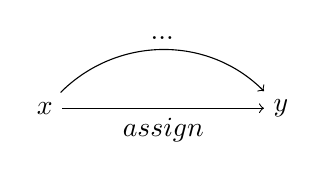
\begin{tikzpicture}[node distance=3.0cm] 
          \node[] (1) {$x$};
          \node[] (2) [right of=1] {$y$};
          
          \draw[->] (1) to [out=45, in=135, looseness=1] node[midway, above] {$...$} (2);
          \draw[->] (1) to node[midway, below, sloped] {$assign$} (2); 
    \end{tikzpicture} 
    &
    z = y; x = z;
    & 
    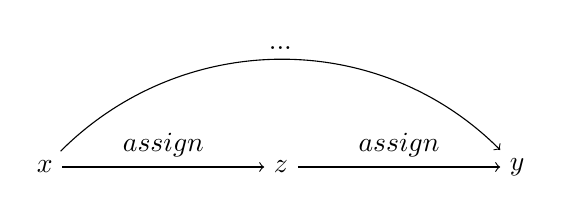
\begin{tikzpicture}[node distance=3.0cm] 
          \node[] (1) {$x$};
          \node[] (2) [right of=1] {$z$};
          \node[] (3) [right of=2] {$y$};
          
          \draw[->] (1) -- node[midway, above, sloped] {$assign$} (2); 
          \draw[->] (2) -- node[midway, above, sloped] {$assign$} (3); 
          \draw[->] (1) to [out=45, in=135, looseness=1] node[midway, above] {$...$} (3);
    \end{tikzpicture} 
    \\
    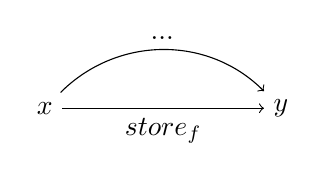
\begin{tikzpicture}[node distance=3.0cm] 
          \node[] (1) {$x$};
          \node[] (2) [right of=1] {$y$};
          
          \draw[->] (1) to [out=45, in=135, looseness=1] node[midway, above] {$...$} (2);
          \draw[->] (1) to node[midway, below, sloped] {$store_f$} (2); 
    \end{tikzpicture} 
    &
    z = y; x.f = z;
    & 
    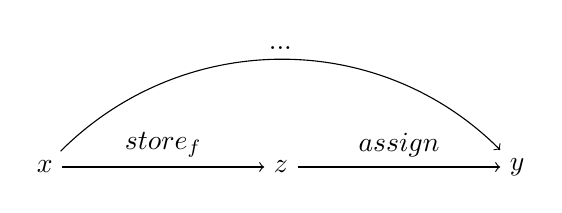
\begin{tikzpicture}[node distance=3.0cm] 
          \node[] (1) {$x$};
          \node[] (2) [right of=1] {$z$};
          \node[] (3) [right of=2] {$y$};
          
          \draw[->] (1) -- node[midway, above, sloped] {$store_f$} (2); 
          \draw[->] (2) -- node[midway, above, sloped] {$assign$} (3); 
          \draw[->] (1) to [out=45, in=135, looseness=1] node[midway, above] {$...$} (3);
    \end{tikzpicture} 
    \\
    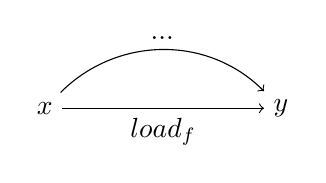
\begin{tikzpicture}[node distance=3.0cm] 
          \node[] (1) {$x$};
          \node[] (2) [right of=1] {$y$};
          
          \draw[->] (1) to [out=45, in=135, looseness=1] node[midway, above] {$...$} (2);
          \draw[->] (1) to node[midway, below, sloped] {$load_f$} (2); 
    \end{tikzpicture} 
    &
    z = y.f; x = z;
    & 
    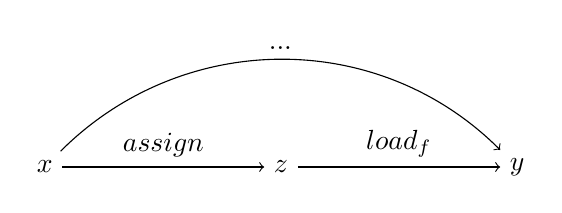
\begin{tikzpicture}[node distance=3.0cm] 
          \node[] (1) {$x$};
          \node[] (2) [right of=1] {$z$};
          \node[] (3) [right of=2] {$y$};
          
          \draw[->] (1) -- node[midway, above, sloped] {$assign$} (2); 
          \draw[->] (2) -- node[midway, above, sloped] {$load_f$} (3); 
          \draw[->] (1) to [out=45, in=135, looseness=1] node[midway, above] {$...$} (3);
    \end{tikzpicture} 
    \end{tabular}
    \caption{Адаптация графа}
  \label{fig:java_graph_transform}
\end{figure}


Поскольку для пересечения автомата и графа применяется произведение Кронекера, необходимо задать бинарную операцию умножения для элементов матриц смежности описанного формата. Если ребро в графе и ребро в автомате содержат одинаковый нетерминал или одинаковый терминал, то соответствующая ячейка в результате произведения Кронекера будет $true$, иначе --- $false$. Эту операцию можно задать так: $times(x, y) = (x_{nonterm} = y_{nonterm} \neq 0 \ or\ x_{term} = y_{term} \neq 0)$. Данное представление графа и рекурсивного автомата в виде матриц с применением такой операции позволяет на каждой итерации алгоритма вычислять произведение Кронекера всего один раз.

\subsection{Применение модификации для анализа псевдонимов}

На рис.~\ref{fig:ma_rsm} представлен рекурсивный автомат для анализа псевдонимов. В нём переход между любыми двумя состояниями происходит только по одной метке, поэтому для него можно использовать описанное выше представление. Однако в результате анализа между двумя вершинами могут быть добавлены как ребро $MA$, так и ребро $VA$. Поэтому необходимо иметь возможность хранить два нетерминала на ребре.

\begin{figure}[h]
  \begin{tabular}{|c|c|}
    \hline
    MA & VA \\
      % Программа & Граф выражений \\
      
      \begin{minipage}{.53\textwidth}
      \scalebox{0.7}{
      \begin{tikzpicture}[node distance=1.9cm, auto] 
          \node (q0) [state, initial, initial text = {}] {$q_0$};
          \node (q1) [state, right = of q0] {$q_1$};
          \node (q2) [state, right = of q1] {$q_2$};
          \node (q3) [state, accepting, right = of q2] {$q_3$};
          
          \path [-stealth, thick]
              (q0) edge node[above] {$\overline{d}$} (q1)
              (q1) edge node[above] {$VA$} (q2)
              (q2) edge node[above] {$d$} (q3)
              ;
      \end{tikzpicture}
      }
      \end{minipage}
  
      &
  \begin{minipage}{.43\textwidth}
  \scalebox{0.7}{
      \begin{tikzpicture}[node distance=2.8cm, auto] 
          \node (q0) [state, accepting, initial, initial text = {}] {$q_4$};
          \node (q1) [state, accepting, right=4.7cm of q0] {$q_5$};
          \node (q2) [state, accepting, below = of q0] {$q_6$};
          \node (q3) [state, accepting, below = of q1] {$q_7$};
          
          \path [-stealth, thick]
              (q0) edge node[above] {$a$} (q1)
              (q0) edge [loop above] node[above] {$\overline{a}$}()
              (q0) edge[bend right] node[left] {$MA$} (q2)

              (q1) edge[loop above] node[above] {$a$}()
              (q1) edge[bend right] node[left] {$MA$} (q3)

              (q2) edge[bend right] node[right] {$\overline{a}$} (q0)
              (q2) edge node[below] {$a$} (q1)
              
              (q3) edge[bend right] node[right] {$a$} (q1)
              ;
      \end{tikzpicture} 
      }
      \end{minipage}
      \\
      & \\
      \hline
  
  \end{tabular}
  \caption{Рекурсивный автомат для анализа псевдонимов}
  \label{fig:ma_rsm}
\end{figure}


Чтобы хранить несколько нетерминалов на ребре, старшие биты числа, содержащего информацию о ребре, будут содержать не номер нетерминала, а маску для всех возможных нетерминалов. Тогда можно задать операцию умножения элементов для произведения Кронекера так: $times(x, y) = (x_{nonterm} \& y_{nonterm} \neq 0 \ or\ x_{term} = y_{term} \neq 0)$.


Стоит отметить, что такое представление также подойдёт для Points-to анализа, учитывающего поля, но оно потребует отдать под нетерминалы на один бит больше. Это может негативно сказаться на потреблении памяти: если под хранение терминала в числе не будет хватать памяти, придётся брать более длинный целочисленный тип для хранения.


\subsection{Особенности реализации}

Данная модификация тензорного алгоритма и её инкрементальная версия были реализованы в библиотеке CFPQ\_PyAlgo\footnote{\url{https://github.com/FormalLanguageConstrainedPathQuerying/CFPQ_PyAlgo/tree/vkutuev/ot_tensor}, пользователь vkutuev. Дата посещения 22.05.2023}, в которой для работы с разреженными матрицами используется библиотека pygraphblas, являющаяся python-обёрткой над библиотекой SuiteSparse. 

При использовании предложенной операции умножения элементов матрицы после произведения Кронекера большинство элементов матрицы-результата будут $false$. Это приводит к двум проблемам: 
\begin{enumerate}
    \item вычисление транзитивного замыкания потребует больше времени, так как матрица содержит больше элементов;
    \item необходимо выделить больше памяти под хранение этой матрицы.
\end{enumerate}

Очистка матрицы от значений $false$ после транзитивного замыкания поможет решить первую проблему. Однако потребность выделить дополнительную память под незначащие элементы матрицы может привести к нехватке памяти. 

Для решения этой проблемы были внесены изменения в исходный код функции, вычисляющей произведение Кронекера, в библиотеке SuiteSparse\footnote{\url{https://github.com/vkutuev/GraphBLAS/tree/vkutuev/kron}, пользователь vkutuev. Дата посещения 22.05.2023}: перед выделением памяти под матрицу-результат производится вычисление количества значащих элементов в результате, и выделение памяти происходит только под это число элементов. Благодаря этому подходу удалось снизить пиковое потребление памяти. На рис.~\ref{fig:memory_profile_a} представлен профиль памяти работы алгоритма со стандартной реализацией произведения Кронекера из библиотеки SuiteSparse с последующей фильтрацией результата, пиковое потребление памяти --- 5,2 ГиБ. А на рис.~\ref{fig:memory_profile_b} --- профиль памяти работы алгоритма с доработанной реализацией, выделяющей память только под элементы результата, которые будут $true$, пиковое потребление памяти --- 2,3 ГиБ.

\begin{figure}[]
    \begin{subfigure}{\textwidth}
        \centering
        \includegraphics[width=\linewidth]{figures/mem_prof_base.pdf}
        \caption{Стандартная реализация}
        \label{fig:memory_profile_a}
    \end{subfigure}
    \begin{subfigure}{\textwidth}
        \centering
        \includegraphics[width=\linewidth]{figures/mem_prof_patched.pdf}
        \caption{Оптимизированная реализация}
        \label{fig:memory_profile_b}
    \end{subfigure}
    \caption{Профиль потребления памяти на одном графе с разными реализациями произведения Кронекера}
    \label{fig:memory_profile}
\end{figure}

